\begin{frame}
	\frametitle{Background: ESRC Advanced Training Initiative}

	\begin{itemize}

		\item The Advanced Training Initiative (\ati) by the Economic
			and Social Research Council (\esrc) provided grants to
			support training in advanced social science topics.

		\item We were funded to provide a series of workshops on Bayesian data analysis each year for the years 2015, 2016, \& 2017:\\
			{\begin{center}\texttt{http://www.priorexposure.org.uk}\end{center}}

		\item Each workshop was limited to around 25 attendees, and could be attended by any UK based social science researchers (post-graduate students and above).

		\item We taught 4 workshops in 2015, 9 in 2016, and 9 in 2017

	\end{itemize}

\end{frame}

\begin{frame}
	\frametitle{Our case for support}
		Bayesian methods are growing in popularity, but are not yet part of the social science curriculum.

		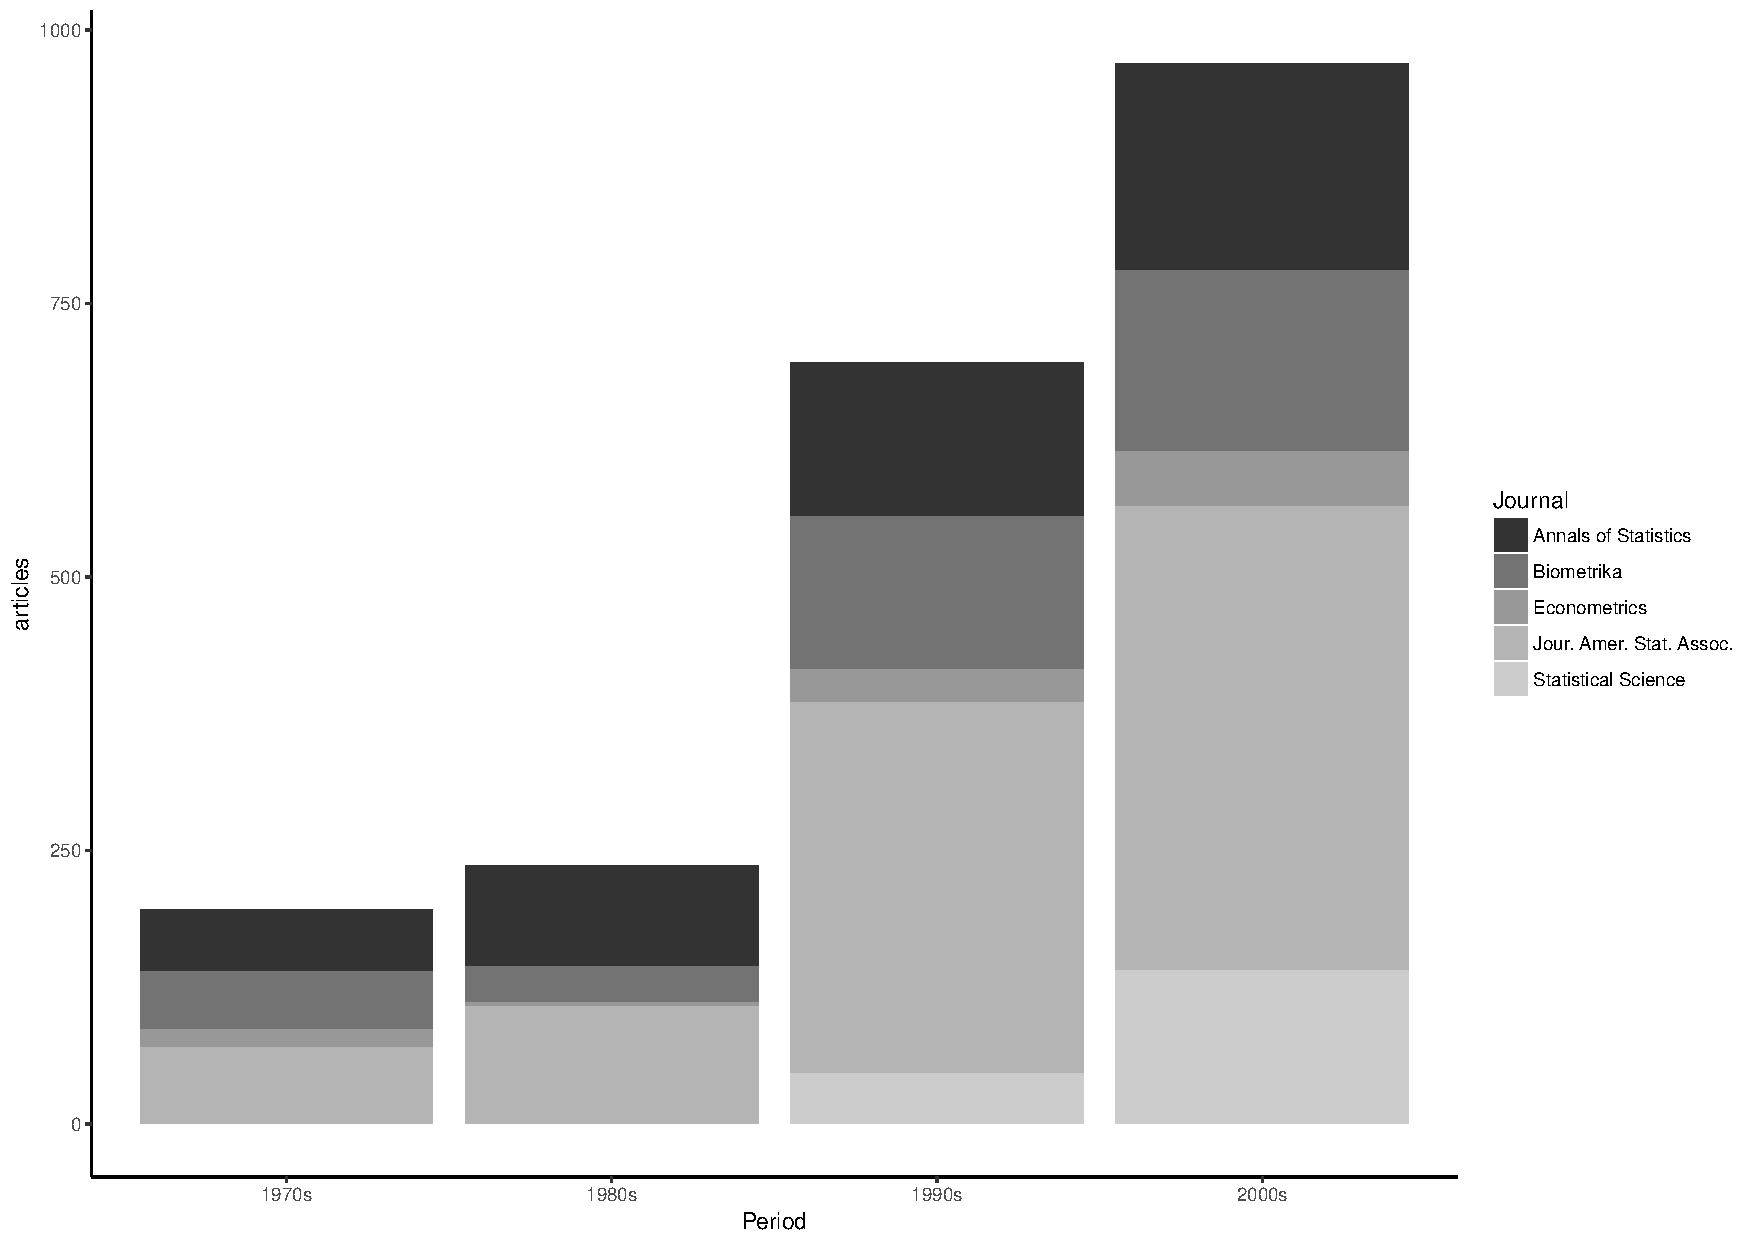
\includegraphics[width=\textwidth]{articles.pdf}
\end{frame}

\begin{frame}
	\frametitle{Our case for support}

		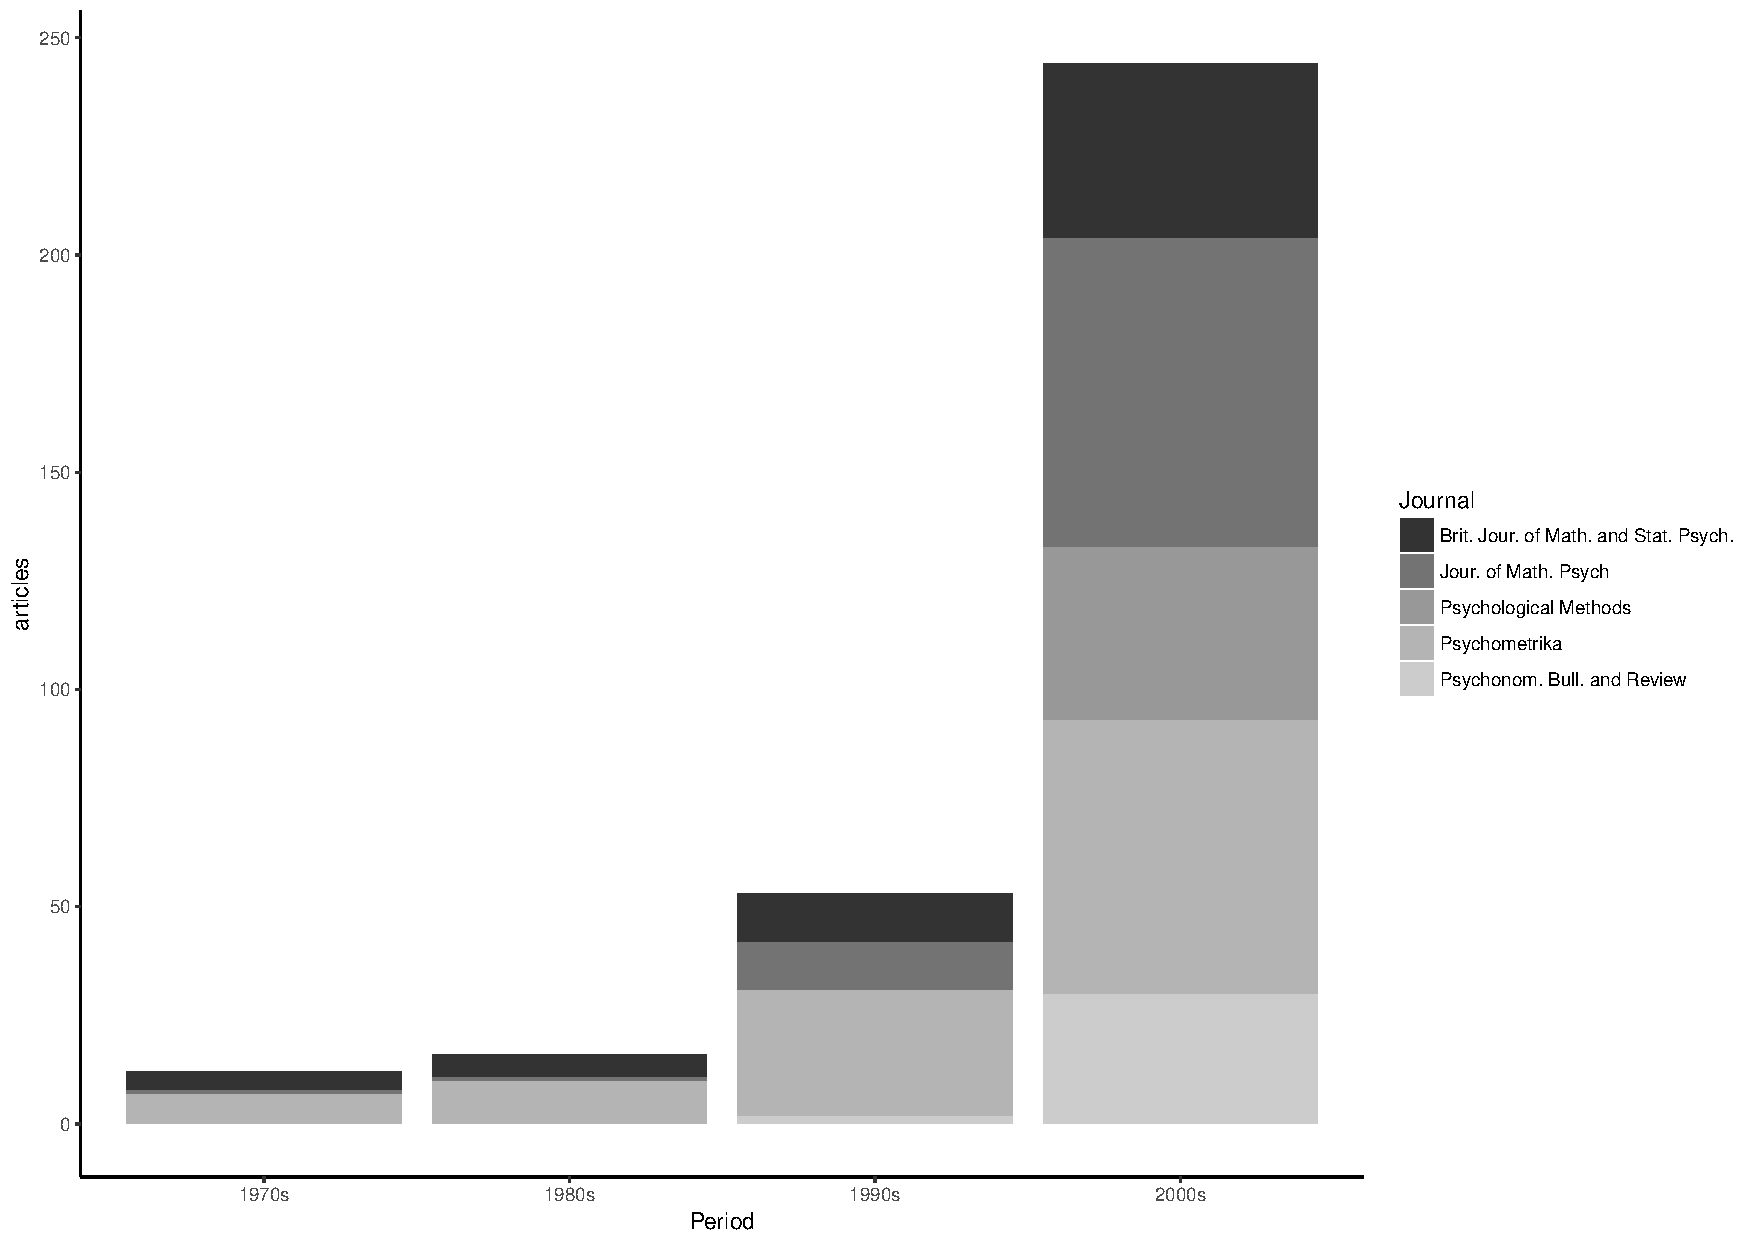
\includegraphics[width=\textwidth]{psyarticles.pdf}
\end{frame}



%	\begin{itemize}
%
%		\item The Advanced Training Initiative (\ati) by the Economic
%			and Social Research Council (\esrc) provided grants to
%			support training in advanced social science topics.
%
%		\item Professor Thom Baguley (\faTwitter \texttt{@seriousstats})  and I were funded to provide a series of workshops on Bayesian data analysis each year for the years 2015, 2016, \& 2017:\\
%			{\begin{center}\texttt{http://www.priorexposure.org.uk}\end{center}}
%
%		\item Each workshop was limited to around 25 attendees, and could be attended by any UK based social science researchers (post-graduate students and above).
%
%		\item There was a minimal fee of \pounds20 per workshop, with a \pounds10 fee for students. There were bursaries to support travel and accommodation expenses by students.
%
%		\item We taught 4 workshops in 2015, 6 (or 9) in 2016, and will teach 6 (or 9) in 2017\footnote{The reason for and details of the extra workshops in 2016 and 2017 will be explained.}.
%
%	\end{itemize}

